\chapter{Introduction}\label{chap:introduction}

\chapterQuote{\textit{``Above all, don't fear difficult moments. The best comes from them.''}}{--- \textit{Rita Levi-Montalcini}}

\chapterAbstract{T}{he purpose of this book is to present our work in Knowledge Graph reasoning. This chapter provides the required information for the reader to follow the topics discussed in this dissertation, it is structured in the following sections: 

Section~\ref{sec:intro-context}, contains the reasons why we found the works we introduce could contribute to the current state of these research fields; 
Section~\ref{sec:intro-rationale}, holds our hypothesis and thesis; 
Section~\ref{sec:intro-summary}, focuses on the contributions made and what they present;
Section~\ref{sec:intro-structure}, describes the structure of the rest of this book.}

\section{Research context}\label{sec:intro-context}

In the last decade, available information online has increased 60 000\%, from a modest 2 zettabytes of data ($10^{12}$ gigabytes) up to an estimate of 120 by the end of 2023\cite{Marr2021}. The sheer volume of being generated on a daily basis calls for a structured and networked storage solution made possible by Knowledge Graphs, whose rise to popularity was all but inevitable. 
These data structures hold information from multiple domains by using triples, two information nodes that represent concepts connected by an edge constituting a relationship between them, this relation can be either directional or linear meaning that a concept is related to another following that direction but not vice-versa, (e.g. parents and children are directional relations while siblings are linear).
This form of representation obtained by adhering to these rules confers information in a graph-like structure containing a web of facts with a high degree of connectivity, offering complex reasoned chains of information in an effective way.

\begin{figure}[!htp]
    \centering
    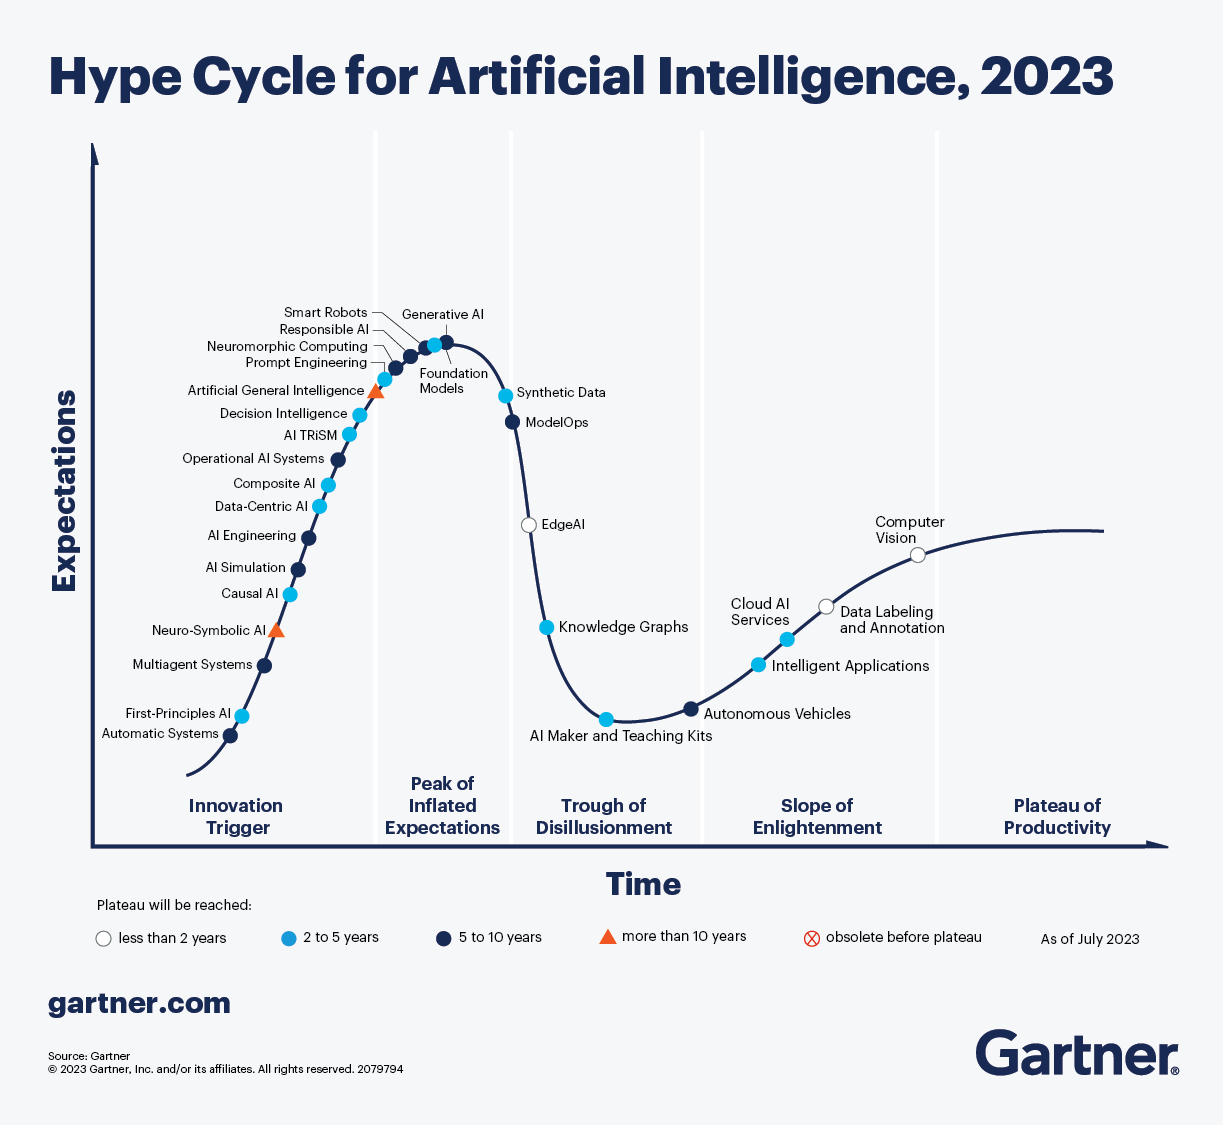
\includegraphics[width=\textwidth]{fig/intro/Gartner_2023.png}
    \caption{Gartner's 2023 hype chart for artificial intelligence.}
    \label{fig:garter-chart}
\end{figure}

The Gartner institution places Knowledge Graphs in the middle of their life cycle (cf. Figure \ref{fig:garter-chart}) meaning that they can still benefit from active research and development and are still in their infancy in regard to their widespread applications in a multitude of fields. Some of the most notable fields and Knowledge Graphs corresponding to each of them are:
\begin{itemize}
    \item \textbf{Enciclopedic} KGs compile factual knowledge facts or events sourced from different domains. Some examples are DBpedia\cite{auer2007dbpedia} which compiles the knowledge found in Wikipedia articles, Freebase\cite{bollacker2007freebase} which combines automatic processes from multiple sources as well as user contributions to wrangle up its data or YAGO\cite{suchanek2007yago} which adds a layer of complexity by adding temporal and geographical information to Wikipedia facts.
    \item \textbf{Linguistic} KGs compile facts about language and add a layer of information in the form of ontologies or external features on top. The most notable of these is WordNet\cite{miller1995wordnet} which provides hyponym and synonym relationships between words of the English language.
    \item \textbf{Enterprise} KGs support tech sector companies in their endeavors. Knowledge graphs were originally conceived for this purpose as the Google Knowledge Graph (GKG) \cite{steiner2012adding} boasting an impressive 800 billion facts on 8 billion entities was incepted to aid in query answering. This graph compiles multi-domain information in order to rapidly respond to one of the many user queries made through their browser per day. 
    
\end{itemize}

Knowledge Graph construction is generally an automatic task since the large volume of data they hold extends past the range of human processing abilities. Manually constructing a KG of large size becomes an exceptionally tedious, long, and costly process, or even downright impossible. However, there are some notable exceptions such as the high-quality datasets that were constructed through crowdfunding efforts such as Freebase\cite{bollacker2007freebase} and Wikidata\cite{vrandevcic2014wikidata}. Automatic KG construction typically relies on semi-structured\cite{lehmann2015dbpedia} information ranging from XML-type documents and HTML tables to plain text articles with a well-organized title structure.
The data extraction process has evolved over time, from information extraction systems driven by designated rules or clustering \cite{yates2007textrunner, etzioni2004web}, to the current approaches such as entity recognition\cite{huang2015bidirectional, ma2016end}, typing\cite{xu2018neural, ren2016label} and linking\cite{ganea2017deep, le2018improving} or relation extraction and curation\cite{zeng2015distant, zhou2016attention}. 

These methods of automated construction allow for a massive volume of data to be processed, however, they present several limitations.
First, the information they are built upon may be interpreted and linked erroneously or simply be demonstrably wrong \cite{martinez2020information}, leading to incorrect facts being present in a KG. 
Second, Knowledge Graphs built from the same source might not be equal rendering them incompatible, they could represent the same facts with different nomenclature because they used a different schema to link that information \cite{choi2006survey}, meaning that integrating Knowledge Graphs is never a trivial task.
Finally, Knowledge Graphs constructed in this manner will most likely be lacking information that was originally contained within the source material it used \cite{bordes2014constructing}. In addition, information sources generally do not include knowledge that the intended reader should already be aware of, in other words, no source will explicitly hold all information required for a single domain, therefore, Knowledge Graphs inherently lack triples that could otherwise exist in them.
Some techniques aim to fill this information gap in automatically constructed Knowledge Graphs, known as KG completion, and their focus is on finding links between existing entities that are not present in the KG but should be. However, KG completion efforts have a limitation shared by multiple binary classifiers in the literature, they generally provide an answer to a query that can be accompanied by a degree of confidence in the form of a percentage. This lack of explainability of their answers is a limitation in KG completion that KG reasoning aims to complement by providing reasoned paths to accompany their responses. In this way, a provided answer can be human-friendly as well as serve the same purpose in regards to KG completion.

Existing literature displays the multiple ways in which KG completion and reasoning have been tackled. Completion efforts can be separated into one of four existing categories\cite{shen2022comprehensive}, they are as follows.
\textbf{Semantic matching models}, compute a scoring function by measuring the semantic similarities of entity or relation embeddings in latent embedding space, they do so by applying \textbf{Neural Network} or \textbf{Tensor Factorization} models. 
NN models \cite{socher2013reasoning, tran2020multi} present a challenging problem as they require the effective encoding of world knowledge using powerful models that try to approximate human cognition by replicating the neural structures found in our brains. Research has shown that neural networks can capture the semantic features of entities and relations intelligently and model the semantic relationships between discrete entities, ultimately leading to more accurate embeddings of KGs.
Tensors\cite{nickel2011three, balavzevic2019tucker, socher2013reasoning, } and their decompositions are widely used in data mining and machine learning problems. their usefulness comes from the representation they offer as KG entities and triples can be represented as tensors, KG completion can be tackled as a binary tensor completion problem\cite{shen2022comprehensive}.

\textbf{Translational models}\cite{bordes2013translating, wang2014knowledge, lin2015learning, sun2019rotate, trouillon2016complex, dettmers2018conve} encode KG entities and relations as low-dimensional numerical vectors. a distance scoring function is then applied in the N-dimensional vectorial space reflecting the correctness of a proposed triple, then a ranking loss function is applied to learn the top translation relation between the entities in question.
\textbf{Structural models}\cite{mikolov2013efficient, pennington2014glove} The inherent rich information inside KGs plays an important role in capturing useful features of knowledge embeddings for KG completion. the common internal information inside KGs includes node attribute information, entity-related information, relation-related information, neighborhood information, and relational path Information. This dissertation's proposal expands on relational path reasoning combined with translational elements as part of the contribution.

% This needs to be formalized, cited, completed and improved...

Obtaining information from relational paths contained within a KG is usually performed by applying machine learning algorithms; path capture, path classification\cite{xiong2017deeppath}, path augmentation\cite{manchanda2023metapath, hirose2021transductive} or multi-hop KG reasoning\cite{lin2018multi, tiwari2021dapath, cui2023incorporating, cui2023reinforcement}. Most of these approaches present an inherent flaw, they use a path ranking NN as a binary classifier which causes feature explosion for large KGs and lacks background information on the selected path, both of those shortcomings are solved by KG reasoning methods. That is why in our works we focused on the development of a multi-hop reasoning approach that adds explainability and prevents feature explosions for large KGs.

There are several options for the construction of artificial intelligence capable of performing KG reasoning, namely, supervised, unsupervised and reinforcement learning.

Supervised learning requires providing a golden truth in a labeled dataset, which means knowing the optimal outcome beforehand, this is useful for tasks that require classification and regression problems, predicting a value in continuous or discrete spaces. This is simply not possible for many problems in the field, in this case, it would mean obtaining the best path connecting two given nodes of a Knowledge Graph for the particular problem being solved. This would require expert knowledge and deep analysis for each of the nodes, a task which is simply unfeasible for sizeable Knowledge Graphs.

% In unsupervised learning no labeled dataset is provided it tries to learn the the underlying patterns of the problem and in this way approximate the output, however, traditional unsupervised approaches often struggle to handle the complexity of real-world knowledge graphs, especially when faced with missing or ambiguous information

Unsupervised learning operates without a labeled dataset, aiming to discern underlying patterns within a problem and approximate the output. However, traditional unsupervised methods frequently encounter challenges in managing the intricacies of real-world knowledge graphs, particularly when confronted with ambiguous or missing information.

Reinforcement learning (RL) emerges as a promising paradigm to address these limitations. RL introduces an interactive learning framework where an agent learns to navigate and interact with the knowledge graph by using it as the environment of the problem. RL algorithms can dynamically adapt their strategies, effectively dealing with the uncertainties present in an automatically constructed KG even in the absence of human supervision.

In practice, Reinforcement Learning focuses on solving a stochastic gradient ascent problem in a KG reasoning scenario, that will be described in depth in chapter \ref{chap:reinforcement}, it is a policy gradient method seeking to optimize the quality of the found path based on the metrics of some reward functions. 

It does so by traversing through the graph nodes as states by using connected relations as the action space for that state. The objective of the Agent is to learn the best path that answers a particular query. This query can be interpreted in the form of a question that needs answering, such as, ``who is the partner of Keanu Reeves?'' This, in the KG nomenclature, is expressed as a triple missing its end node (Keanu Reeves, is\_partner\_of, ?), the agent is then expected to find the destination node while training in order to generate new paths of information from the unanswered queries contained in the KG.

Several proposals have tackled this problem in the past \cite{xiong2017deeppath, das2017go, lin2018multi, xian2019reinforcement}. However they present several shortcomings, for instance, they require the embedding models to be computed before attempting the problem. Also, they restrict themselves to using classical RL backpropagation algorithms and overlook the application of more modern options such as Proximal Policy Optimization (PPO)\cite{schulman2017proximal} or Soft Actor-Critic (SAC) \cite{haarnoja2018soft} while also relying on simple reward structures. Finally, most of these proposals are not distributed as usable tools intended for final users. Even if they make their implementation publicly available, their code is generally intended for the sake of reproducibility of their experimental results, and they often lack any degree of customization or flexibility, meaning they usually can only work on a number of predefined datasets as input.

In this dissertation work, we aim to combine the benefits from RL pathfinding with the power of representational embeddings to infer fairly long and explainable paths, useful for KG-based applications, and doing so with on-the-fly embedding generation and embedding-based rewards combined with step-based rewards.

The tool presented is highly configurable, allowing for reward calculation to be modified with a combination of several options, customizing the policy intermediate activation function and regularization and allowing the user to apply state-of-the-art RL algorithms out of the box, which improves performance and helps avoid reward plateaus while training.

Finally, we aim to provide a versatile tool intended for users with different levels of expertise, from novices to experts. It allows comprehensive and flexible customization for advanced users, who may prefer to install SpaceRL as a server for their local usage or to become a service provider for third parties. On the other hand, it also offers a simple MLaaS interface, intended for a more untrained end user. Machine Learning as a Service (MLaaS) has gained traction in recent years since it adds layers of abstraction that create a black-box simplified interface for a non-expert final user. SpaceRL offers RL model generation and usage as a service capability, either locally through its GUI or as a deployable REST API for third-party consumption. Therefore, it is, to the best of our knowledge, the first turnkey tool to provide such RL KG completion and reasoning functionalities.

\section{Research rationale}\label{sec:intro-rationale}
In this section, we present the hypothesis that has motivated our research work in the context of Knowledge Graph reasoning and state our thesis, which we prove in the rest of the dissertation.

\subsection{Hypothesis}
% \todo{En mi opinion aqui no solo debemos hablar de la oportunidad que suponen los grafos de conocimiento como tal y por eso hay que completarlos, si no de lo que supone mejorar la accesibilidad de las prpuestas que lo ofrecen, porque tambien forma parte de la tesis, no creo por tanto que la mencion a la limitacion de las técnicas sobre de aqui.}

Currently, Knowledge Graphs present a tantalizing alternative for structuring information about one or multiple domains. They offer a semantic connection between the data nodes which can be used for a multitude of applications such as question answering \cite{cui2023incorporating, cui2023reinforcement}, recommendation systems \cite{xian2019reinforcement}, biomedical studies \cite{nicholson2020constructing} or natural language processing tasks. The nature of these knowledge graphs makes them inherently incomplete as their construction is often automatic, granting for their expansion with a variety of techniques. 
however, these techniques \cite{bordes2013translating, wang2014knowledge, lin2015learning, sun2019rotate, trouillon2016complex, nickel2011three, balavzevic2019tucker, socher2013reasoning, lao2011random, das2017go, xiong2017deeppath, lin2018multi, xian2019reinforcement, tiwari2021dapath} come with their own set of limitations, most notably how they provide close to no input about why they provided the results they did. In addition, the tools available to perform these tasks are limited due to the nature of their conception, created to test a specific technique and made available for replication purposes only by expert users, as opposed to being designed with usability and customization in mind.

According to the previous argumentation, we conclude that our hypothesis is the following:

% Knowledge Graphs provide value to individuals and companies alike by supporting applications that are widely used today, and their usefulness is likely to keep growing. Due to their incompleteness, there is a need to refine them and find the information that they are missing in order to expand them.

\hypthesis{Knowledge Graphs provide a way to structure information such that it provides semantic value to applications that rely on them and are widely used. They are inherently incomplete and can be expanded, however, the methods that do so are limited in two major ways, they lack explainability for the generated knowledge and are only usable for expert users, if at all.}

\subsection{Thesis}

% \todo{estoy de acuerdo en que esto le falta contexto en algun momento, lo reescribiré.}

A multitude of approaches have tackled the problem of KG completion \cite{bordes2013translating, wang2014knowledge, lin2015learning, sun2019rotate, trouillon2016complex, nickel2011three, balavzevic2019tucker, BorregoAHRR21, Sola2023AYNEXT} and reasoning \cite{socher2013reasoning, lao2011random, das2017go, xiong2017deeppath, lin2018multi, xian2019reinforcement, tiwari2021dapath, cui2023incorporating, cui2023reinforcement}. Triple \textbf{classification} KG completion methods aim to classify new triples as true or false to include them in the graph, hence completing them, however, these methods lack explainability for their results and do not provide any knowledge apart from a certain degree of confidence.
On the other hand KG \textbf{reasoning} approaches do provide an explanation for how they reached their results and they do so by applying a plethora of algorithms and techniques that are not without their own limitations. Their reward structures are based on the retropropagation of simple terminal rewards that require the learning Agent to reach a particular state to progress. They also suffer from highly variable inference accuracy caused by the RL algorithms used. They often disregard the semantic value of the vectorial representations they use for the nodes and relations and only apply them as the input of NN classifiers. Finally, existing techniques could be updated or expanded by domain experts if their construction granted for it, however, the tools presented are almost always tailored for the only purpose of producing results for publication and nothing more, and this generally means making them hard to work with and expand.

In light of the previous reasoning, we conclude that our thesis is as follows:

% In the context of Knowledge Graph completion, it is possible to overcome the problems of existing proposals and develop a new one to automatically complete the missing information in a large KG, in a way that does not rely on external information or alternative representations, but that still achieves a high effectiveness.

\hypthesis{Knowledge graph reasoning can benefit from the development of novel reward structures that leverage the semantic value contained within the embedding representations of graph nodes and relations, more robust Reinforcement Learning algorithms that circumvent the high variance of the methodology of policy gradient methods and from a standardized approach to applying these techniques that focus on ease of expansion, modification and application to make it possible to implement new techniques in the future supported by the same set of tools while also providing support to any user.}

\section{Summary of contributions}\label{sec:intro-summary}
To prove our thesis, we have devised \href{https://github.com/DEAL-US/SpaceRL-KG}{\textbf{\textit{SpaceRL, our KG reasoning framework}}} supported by Reinforcement Learning techniques.

SpaceRL is an end-to-end framework focused on customization and adaptability, it works with any dataset provided in the expected format. SpaceRL allows any user with any level of expertise to generate an intelligent agent able to reason over the KG of their choice in order to generate new knowledge in the form of a triple accompanied by a structured reasoned path.

The framework allows the users to customize it by permitting the tuning of hyperparameters, relying on previous experience with LSTM layers, generating a particular set of embeddings for the dataset being used, using multiple RL algorithms, reward structures and depth of reasoned paths.

It also allows for the deployment of a relation API in order to be a service provider for tuned models or to provide infrastructure for model generation to a third party, as well as offering a GUI in order to give inexperienced users a comprehensive view of the system for them to generate models and tune them as needed, without expert knowledge of the field. The system also offers visualization tools that give the user an overview of how the trained models choose the paths while in inference mode in order to better understand the decisions made.

SpaceRL is meant to be easily expanded, however, it also comes with multiple options out of the box, we have mentioned in the introduction how current KG reasoning approaches are lacking in inference stability, which is why SpaceRL defaults to the usage of the Proximal Policy Optimization (PPO) reinforcement learning algorithm and comes out of the box with novel reward structures based on the properties of the embeddings for the evaluated KG. these options were used in our paper "SpaceRL-KG: Searching Paths Automatically Combining Embedding-based Rewards with Reinforcement Learning in Knowledge Graphs", currently under review in Expert systems with applications. The framework, complete with API and GUI has been sent to SoftwareX, and is currently awaiting to be reviewed by the editor.

\section{Structure of this dissertation}\label{sec:intro-structure}
This dissertation is structured as follows:

\begin{description}
    \item[\textbf{Part I: Preface.}] 
    It holds the introductory chapters to this dissertation, the one holding these words plus Chapter \ref{chap:motivation}, where we go into detail about the justification that granted the works presented in this book, presenting the limitations of the current state-of-the-art approaches.\\
    
    \item[Part II: Background Information.] 
    This Part gives insight into the topics necessary to better understand the proposals presented, In chapter \ref{chap:kgs} we give an overview of Knowledge graphs, how they are structured, constructed, applied and the challenges in the field. In chapter \ref{chap:embeddings}, we introduce the representational techniques for knowledge graphs known as embeddings, how they work and several proposals that apply the different techniques used to generate them. In chapter \ref{chap:reinforcement} we give an introduction to Reinforcement Learning, how it can solve KG reasoning tasks and how it operates within the scope of a knowledge graph, the evolution of the techniques and algorithms and how each of them operates and some applications RL has had success on.
    
    \item[Part III: Our Proposal.]
    This Part reports on the contributions made in this dissertation. In chapter \ref{chap:SpaceRL} we describe the methodology followed to create reinforcement learning agents and how they fared on several state-of-the-art datasets to generate reasoned paths following our new reward structure and use of modern RL algorithms. In chapter \ref{chap:framework} we present our framework for RL-based KG reasoning tasks, how it works and the advantages it poses over creating new one-time use code for a proposal, how it can help expert users provide a service to others and how can be used by non-expert users.
    
    \item[Part IV: Final Remarks.]
    It contains Chapter~\ref{chap:conclusions}, which concludes this dissertation and presents some possible future research directions.
\end{description}